\section{Peržiūros roboto apžvalga}

Šiame skyriuje analizuojama teorinė saityno peržiūros roboto sistemų medžiaga, esminės funkcinės charakteristikos, nagrinėjamos skirtingos tokių sistemų kategorijos. Skyriaus siekis -- sudaryti skaitytojui aiškesnį probleminės srities kontekstą.

\subsection{Keliavimas žiniatinklio nuorodomis}

Saitynas ir jį sudarantys puslapių ryšiai dažnai apibūdinami pasitelkiant grafų teorijos terminologiją. Galima teigti, jog kiekvienas puslapis yra viršūnė, o nuorodos -- briaunos, kurioms priskiriama kryptis, todėl galima teigti, kad keliavimas žiniatinkliu pasitelkiant žvalgymo robotą yra keliavimas orientuotu grafu \cite{CategoriesOfWebCrawlersAndOverview}. Nuorodos yra paprasčiausi HTML žymėjimo kalbos saitai (angl. \textit{hyperlinks}). Keliavimo strategija tokiose sistemose yra didelė problema, analizuojama ne viename moksliniame straipsnyje. Kaip pastebima iš \ref{fig:graph_structure} paveikslėlio, nuorodos gali būti tiek išorinės (vedančios į kitas svetaines, prisklausančias kitiems saityno serveriams), tiek vidinės, sudarančios svetainės hierarchinę struktūrą.

\begin{figure}[htp!]
\centering
\includegraphics[scale=0.6]{img/grafo_struktūra.png}
\caption{Žiniatinklio grafo struktūros vaizdas}
\label{fig:graph_structure}
\end{figure}

\subsection{Bazinis veikimo algoritmas}

Saityno peržiūros robotų sistemų funkcinis algoritmas nėra sudėtingas -- esminė tokių sistemų užduotis yra turint pradinį URL adresų sąrašą parsiųsti šių puslapių turinį naudojantis HTTP protokolu, iš parsiųstų HTML dokumentų išgauti hipernuorodas ir jas suabsoliutinus (nustačius ir resurso serverio vardą) pridėti į lankytinų nuorodų sąrašą tolesiam žvalgymui \cite{StanfWebCrawl}. Parsiųsti dokumentai saugomi didelėse talpyklose -- tinkle išskirstytose failinėse sistemose ar duomenų bazėse ir gali būti naudojami tolesniam papildomui apdorojimui (pvz.: svetainės indeksavimui ir semantiniam temos nustatymui, didžiųjų duomenų gavybai ir jų struktūrizavimui ar kt.)

Supaprastinta abstrakti tokių sistemų veikimo schema pateikiama \ref{fig:high_level_architecture} paveikslėlyje. Schemoje pastebimas ciklinis veikimo principas -- nuorodos analizuojamos nuolat iki kol ištuštėja lankytinų puslapių sąrašas arba inicijuojamas sistemos darbo nutraukimas iš vartotojo pusės. Tokios sistemos privalo pasižymėti aukštu lygiagretaus agentų veikimo lygiu ir efektyviai išnaudoti sistemos tinklo, procesoriaus ir operatyviosios atminties resursus. Taip pat aktualus ir didelio kiekio duomenų talpinimo klausimas -- saugomi šimtai milijonų dokumentų ir nuorodų, o tai reikalauja didelių talpinimo resursų ir optimalios prieigos prie jų.

\begin{figure}[ht]
\centering
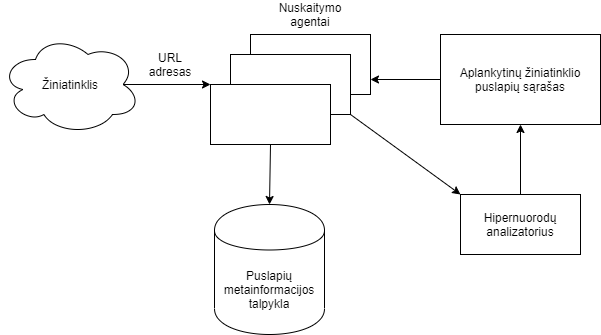
\includegraphics[scale=0.6]{img/Web_Crawler_Architecture.png}
\caption{Aukšto lygio saityno pežiūros roboto architektūra}
\label{fig:high_level_architecture}
\end{figure}


\subsection{Palyginimas su saityno duomenų rinkimo sistemomis}
Terminai \textbf{saityno žvalgymas} (angl. \textit{Web Crawling}) ir \textbf{saityno duomenų rinkimas} (angl. \textit{Web Scraping}) dažnai vartojami kaip sinonimai, nors jų reikšmės skiriasi. Siekiant įvesti aiškią skirtį ir apibrėžti darbe nagrinėjamo tipo sistemų funkcionalumo ribas, šiame skyriuje atliekamas terminų palyginimas. 

\subsubsection{Skirtumai}

Duomenų žvalgymas dažniausiai apima dideles saityno erdves -- vyksta tęstinis procesas, kurio metu siekiama identifikuoti puslapyje pasiekiamas hipernuorodas ir atlikti tų nuorodų tolimesnį žvalgymą. Tuo metu duomenų surinkimo sistema dažniausiai turi aiškų objektą ir jo struktūrą -- konkrečią svetainę ar duomenų bazę ir siekia išgauti tam tikrus dominančius duomenis. Galima teigti, jog saityno žvalgymo sistemos labiausiai suinteresuotos ryšių tarp puslapių nustatymui tam, kad būtų galima keliauti žiniatinkliu, o žiniatinklio duomenų surinkimo sistemų epicentre -- informacijos gavyba \cite{OxylabsScrapingVsCrawling}. \ref{tab:crawling_vs_scraping} lentelėje pateikta keletas esminių lyginamųjų charakteristikų tarp šių vartojamų terminų.

Nagrinėjami terminai skiriasi, tačiau yra itin susiję, nes saityno žvalgymas yra dažniausiai pirmasis informacijos gavybos etapas -- reikalingo turinio surinkimas. Žinoma, duomenų surinkimą galima atlikti be žvalgymo sistemų pagalbos, tačiau žvalgymo sistemos visada kartu naudoja duomenų surinkimo sistemas tam, kad atskirtų vertingą turinį nuo prastos reputacijos svetainės. \cite{OxylabsScrapingVsCrawling}

% Table generated by Excel2LaTeX from sheet 'crawling_vs_scraping'
\begin{table}[htbp]
  \centering
  \caption{Duomenų žvalgymo ir surinkimo sistemų palyginimas \cite{PromptCloudScrapingVsCrawling}}
    \begin{tabular}{|l|l|p{13.57em}|}
    \hline
    \textbf{Aspektas} & \textbf{Duomenų žvalgymas} & \textbf{Duomenų surinkimas} \bigstrut\\
    \hline
    Veikimo mastelis & Milžiniškas & Koncentruotas \bigstrut\\
    \hline
    Veikimo erdvė & Žiniatinklis & Žiniatinklis, duomenų bazė, serveris \bigstrut\\
    \hline
    Dublikatų aptikimas & Esminis veiksmas & Nebūtinas veiksmas \bigstrut\\
    \hline
    \multicolumn{1}{|p{12.285em}|}{Esminiai funkciniai komponentai} & Žvalgymo agentai & Žvalgymo agentai ir duomenų analizatoriai \bigstrut\\
    \hline
    Rankinio atlikimo galimybė & Negalima & Galima \bigstrut\\
    \hline
    Tikslas & Hipernuorodų aptikimas & Duomenų išgavimas \bigstrut\\
    \hline
    \end{tabular}%
  \label{tab:crawling_vs_scraping}%
\end{table}%

Šiame rašto darbe nagrinėjamos duomenų peržiūros robotų, dar vadinamų vorais (angl. \textit{Web Spider Bot}), sistemos, kurios keliauja saitynu naudojantis išgaunamomis HTML nuorodomis (angl. -- \textit{anchor tags}). Rašto darbe nėra aptariamas svetainės turinio duomenų apdorojimas, struktūrizuotos informacijos gavyba, nes tai nėra tokių sistemų atsakomybės sritys.

\subsection{Pagrindinės sistemos veikimo politikos}

Saityno peržvalgos roboto sistemų veikimo specifiką sudaro 4 pagrindinių naudojamų strategijų kombinacija. Kiekviena šių politikų yra atskira išsamiai aprašoma mokslinė saityno peržvalgos problema, reikalaujanti nuodugnios analizės, todėl šiuose punktuose šios politikos apžvelgiamos bendrais bruožais.

\subsubsection{Pasirinkimo politika}

Ši politika apibrėžia žvalgytinų puslapių prioritizavimo tvarką. Vienas didžiausių žiniatinklio žvalgymo iššūkių -- milžiniškas Interneto svetainių skaičius, kurio eksponentinis augimas išlieka iki šių dienų. Net patys efektyviausi saityno žvalgymo robotai neturi pakankamai resursų, jog galėtų padengti visas svetaines, todėl atsiranda efektyvaus prioritizavimo klausimas \cite{EffectiveWebCrawling}. Reikalinga efektyvi funkcija, kuri galėtų įvertinti žvalgytino puslapio kokybę dar prieš jį atsisiunčiant. Puslapio kokybę galima suprasti kaip kiekvieną iš šių faktorių:

\begin{itemize}
    \item Nuorodų, rodančių į puslapį, skaičius
    \item Puslapio semantinės temos atitikimas paieškos užklausai
    \item Puslapio semantikos atitikimas nuorodos tekstui
\end{itemize}

\subsubsubsection{Paieška į plotį}

Viena iš paprasčiausių žvalgymo politikų -- paieškos į plotį algoritmas, kurio principas pavaizduotas \ref{fig:bfs} paveikslėlyje. Atlikti eksperimentiniai žvalgymo tyrimai (aplankyta virš 300 mln. svetainių) parodė, jog paieškos į plotį strategija puikiai veikia surenkant aukštos kokybės puslapius žvalgymo pirmuose etapuose \cite{EffectiveWebCrawling}. Ši išvada grįsta nuomone, kad aukštesnės kokybės puslapiai turi daugiau nuorodų, vedančių į juos, todėl atrandami anskčiau \cite{EffectiveWebCrawling}.

\begin{figure}[htp!]
\centering
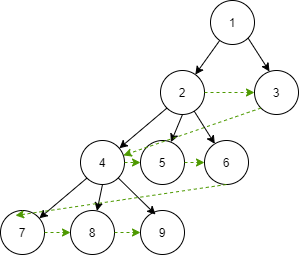
\includegraphics[scale=0.7]{img/BFS.png}
\caption{Paieškos į plotį grafas}
\label{fig:bfs}
\end{figure}

\subsubsubsection{PageRank algoritmo metrika}

Kitas būdas atlikti efektyvesnį žvalgymą -- kiekvienam lanktytinam puslapiui apskaičiuoti kokybės metriką ir lankyti aukštos metrikos vertės puslapius anskčiau. Viena iš tokių metrikų -- „Google“ patentuotas ir šios kompanijos pirmasis svetainių kokybės vertinimo algoritmas „PageRank“.

\begin{figure}[htp!]
\centering
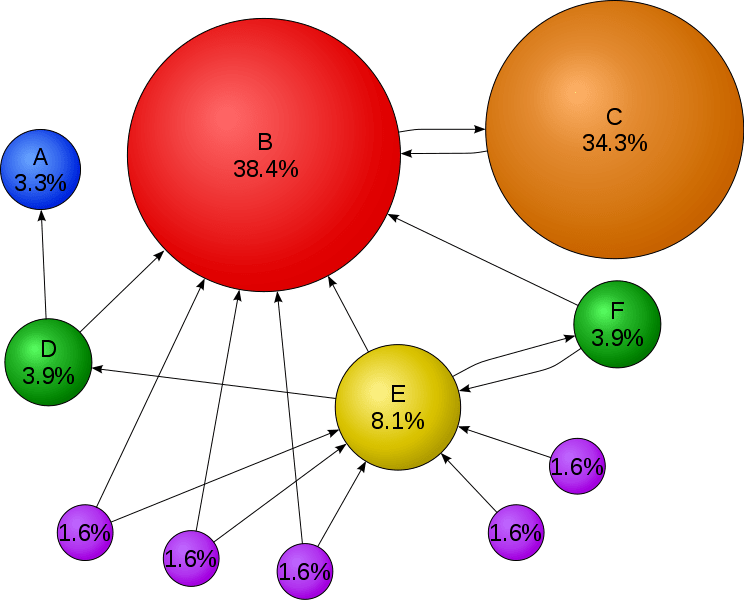
\includegraphics[scale=0.4]{img/pagerank.png}
\caption{„PageRank“ algoritmo principas \cite{PageRank}}
\label{fig:pagerank}
\end{figure}

Kaip galima pastebėti iš \ref{fig:pagerank} grafo, „PageRank“ algoritmas vertina nuorodų skaičių, kurios rodo į tam tikrą puslapį ir tų nuorodų puslapių kokybę. Matoma, jog B viršūnė turi aukštą autoritetą, nes į ją rodo daug mažų viršūnių, o C viršūnė -- nes į ją rodo viena aukšto autoriteto viršūnė.

\subsubsection{Etiško žvalgymo politika}

Saityno žvalgymo robotai veikia naudodami daug lygiagrečių žvalgymo procesų, kurie sugeneruoja didelius kiekius tinklo I/O srauto. Žvalgant konkretų žiniatinklio serverį, svarbu užtikrinti, jog priskirtas žvalgymo procesas nesutrikdytų sklandaus šio serverio darbo, t.y. nesukeltų netyčinės DoS\footnote{DoS - Denial of Service Attack} atakos \cite{EffectiveWebCrawling}. 

\subsubsubsection{REP protokolas}

Kaip dalinė etiško saityno žvalgymo užtikrinimo priemonė, buvo sukurtas \textit{Robots Exclusion Protocol} taisyklių rinkinys, kuriuo svetainių administratoriai gali nurodyti, kurias svetainės dalis jie leidžia robotams pasiekti, taip pat, koks galimas minimalus žvalgymo užklausų laiko intervalas. Pavyzdinis robots.txt failo turinys matomas \ref{fig:rep-example} paveikslėlyje.

\begin{figure}[htp!]
\centering
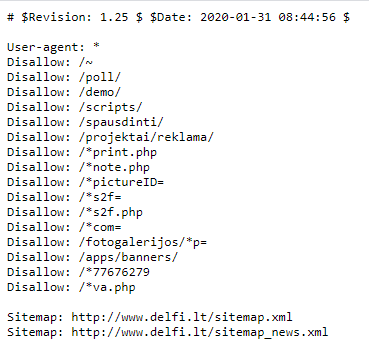
\includegraphics[scale=0.8]{img/rep_protocol.png}
\caption{delfi.lt robots.txt pavyzdys}
\label{fig:rep-example}
\end{figure}

\textit{User-agent} direktyva apibrėžia robotų pavadinimus, kuriems taikomas taisyklių rinkinys. Kiekvienas etiškas žvalgymo robotas kreipdamasis į žiniatinklio serverį identifikuoja save naudodamas šią HTTP antraštės reikšmę. Pavyzdžiui, „Googlebot“ sistema naudoja tokią šios HTTP antraštės reikšmę:
\begin{verbatim}
Mozilla/5.0 AppleWebKit/537.36 (KHTML, like Gecko; compatible; Googlebot/2.1; 
+http://www.google.com/bot.html) Chrome/W.X.Y.Z‡ Safari/537.36
\end{verbatim}
\textit{Disallow} direktyva nurodo, koks dokumentas ar byla negali būti pasiekiama tam tikram robotui. Taip pat gali būti naudojamas „*“ simbolis (\textit{angl. -- wildcard symbol}), nurodantis, jog taisyklių rinkinys turi būti taikomas bet kokiai reikšmei \cite{RobotsExclusionProtocol}.

Į oficialių standartą neįtraukta, bet dažnai sutinkama \textit{Crawl-delay} direktyva, kurią kiekvienas žvalgymo robotas gali interpretuoti skirtingai, dažniausiai tai būna laiko tarpas tarp skirtingų HTTP užklausų į serverį.

Akcentuotina, kad šis protokolas negarantuoja, jog robotas nežvalgys uždraustų direktorijų ar resursų, nes žiniatinklyje yra daugybė neetiškų žvalgymo sistemų, siekiančių blogų tikslų.

\subsubsubsection{Svetainės žvalgymo intervalai}

Ši roboto sistemos charakteristika yra svarbiausia etiško žvalgymo politikoje. Turi būti išlaikytas balansas tarp žvalgymo mandagumo (neapkraunamas žiniatinklio serveris) ir peržvalgos efektyvumo, nes didelės svetainės, turinčios šimtus tūkstančių puslapių, turi būti žvalgomos itin greitai \cite{EffectiveWebCrawling}.

\subsubsection{Pakartotinio apsilankymo politika}

Inkrementinio tipo žvalgymo robotai turi užtikrinti, jog sistemos puslapių indekso repozitorijoje turimos lokalios puslapių kopijos yra kiek galima naujesnės ir atitinkančios originalų resursą esamu laiku. \cite{EffectiveWebCrawling}

Šiam tikslui yra apibrėžtos dvi pagrindinės funkcijos, sutinkamos literatūroje, kurios kartu nusako puslapio pokyčio neaptikimo kainą.

\subsubsubsection{Šviežumo funkcija}

Ši funkcija nusako, ar lokali kopija atitinka originalų resursą duotuoju laiko momentu ir gali būti apibrėžiama taip:

\[F\: p(t) = \left\{\begin{matrix} 1, & p & puslapis & atitinka & laiko & momentu & t\\ 0 & kitu & atveju \end{matrix}\right.\]

\subsubsubsection{Amžiaus funkcija}

Ši funkcija nusako, kokio senumo turima lokali puslapio p kopija:

\[A\: p(t) = \left\{\begin{matrix} 0, & p & puslapis & nepakeistas & laiko & momentu & t\\ t & kitu & atveju \end{matrix}\right.\]

\textit{t} reikšmė šiuo atveju nusako puslapio modifikavimo laiką.

\subsubsubsection{Pakartotinio apsilankymo strategijos}

Pagal \cite{EffectiveWebCrawling} dažniausiai sutinkamos 2 pakaertotinio žvalgymo strategijos:

\begin{enumerate}
    \item Vieningoji strategija -- visi puslapiai pakartotiniai žvalgomi kas tą patį laiko intervalą
    \item Proporcinė strategija -- dažniau kintantys puslapiai žvalgomi dažniau
    \item Svarbos strategija -- svarbesni puslapiai (taikomos metrikos įvertinti, pvz.: „PageRank“) žvalgomi dažniau
\end{enumerate}

Ištirta, jog vieningoji strategija plačiajame žvalgyme efektyvesnė už proporcinę \cite{EffectiveWebCrawling}.

\subsection{Peržiūros robotų kategorijos}

Saityno peržiūros robotų sistemos skirstomas į skirtingas kategorijas pagal taikomas žvalgymo strategijas. Jos bendrai apžvelgiamos šiame poskyryje.

\subsubsection{Teminiai žvalgymo robotai}

Šio tipo (angl. -- \textit{Focused Web Crawlers}) saityno žvalgymo sistemos parsiunčia tik puslapius, atitinkačius specifinę semantinę temą \cite{CategoriesOfWebCrawlersAndOverview}. Puslapiai būna glaudžiai semantiškai susiję vienas su kitu. Tokios sistemos turi sugebėti įvertinti svetainės atitikimą apibrėžtai žvalgymo temai ir nuspręsti, kokiu būdu judėti nuorodų grafu pirmyn. Viena iš pasiūlytų idėjų kaip atpažinti resurso aitikimo žvalgymo roboto temai laipsnį -- HTML žymių (angl. -- \textit{anchor tag}) elemento tekso indeksas ir jo semantinė analizė \cite{AnchorTagsSemanticAnalysis}. Strategijos silpnybė -- svetainių administratoriai lengvai gali manipuliuoti tekstu į resursus, kurie neatitinka žvalgymo robot tematikos.


\subsubsection{Inkrementiniai žvalgymo robotai}

Tradicinės literatūroje aprašytos saityno žvalgymo sistemos periodiškai atnaujina savo turimą žiniatinklio dokumentų indeksą pakeisdamos senus dokumentus naujai parsiųstais \cite{CategoriesOfWebCrawlersAndOverview}. Inkrementiniai robotai savo turimą indeksą keičia analizuodami kiekvieno resurso pokyčio laipsnį (įvairūs semantiniai algorimtai, NPL\footnote{NLP - Natural Language Processing} algoritmai). Tokie robotai taip pat pakeičia mažiau svarbius puslapius į labiau svarbesnius, todėl išsprendžiama indeksuotų resursų naujumo ir aktualumo problema, taip pat taupoma žvalgymo roboto sistemos disko vieta, interneto srautas.

\subsubsection{Išskirstyti žvalgymo robotai}

Ši kategorija labiau apibrėžia žvalgymo roboto sistemos topologinę struktūrą -- sistema susideda iš centrinio serverio, kuris valdo daug išskirstytų agentų: jiems priskiria URL adresus ir liepia atlikti HTTP žvalgybą \cite{CategoriesOfWebCrawlersAndOverview}. Tokios kategorijos sistemos skirtos išgauti plačiam žiniatinklio resursų padengiamumui, šiomis dienomis efektyviam žvalgymui tokia struktūrizacija yra tiesiog privaloma. Taip pat tokios struktūros sistemos yra atsparios tinklo ar serverių darbo nesklandumams, nes pavieniams agentams nutraukus darbą, gali būti priskiriami kiti, nauji lygiagretūs procesai \cite{CategoriesOfWebCrawlersAndOverview}.

\subsubsection{Lygiagretūs žvalgymo robotai}

Kategorija apibrėžia sistemos loginę struktūrą -- agentai gali veikti kaip lygiagrečios gijos, atliekančios HTTP užklausas vienu metu. Ši strategija yra būtina efektyviam puslapių parsiuntimo greičiui per laiko vienetą pasiekti \cite{CategoriesOfWebCrawlersAndOverview}.